\chapter{How to run}
 In order to run the project on android, you need to navigate to the project folder and type in the command as shown below:
 
\begin{lstlisting}
cd ProjectName
npx react-native run-android
\end{lstlisting}

This (in theory) will automatically start the Metro server in another command line console as in Fig.~\ref{fig:Metro}. 

The first time you run the code, the development server (metro) might not start, in that case run the code again.

\begin{figure}[ht]
    \centering
    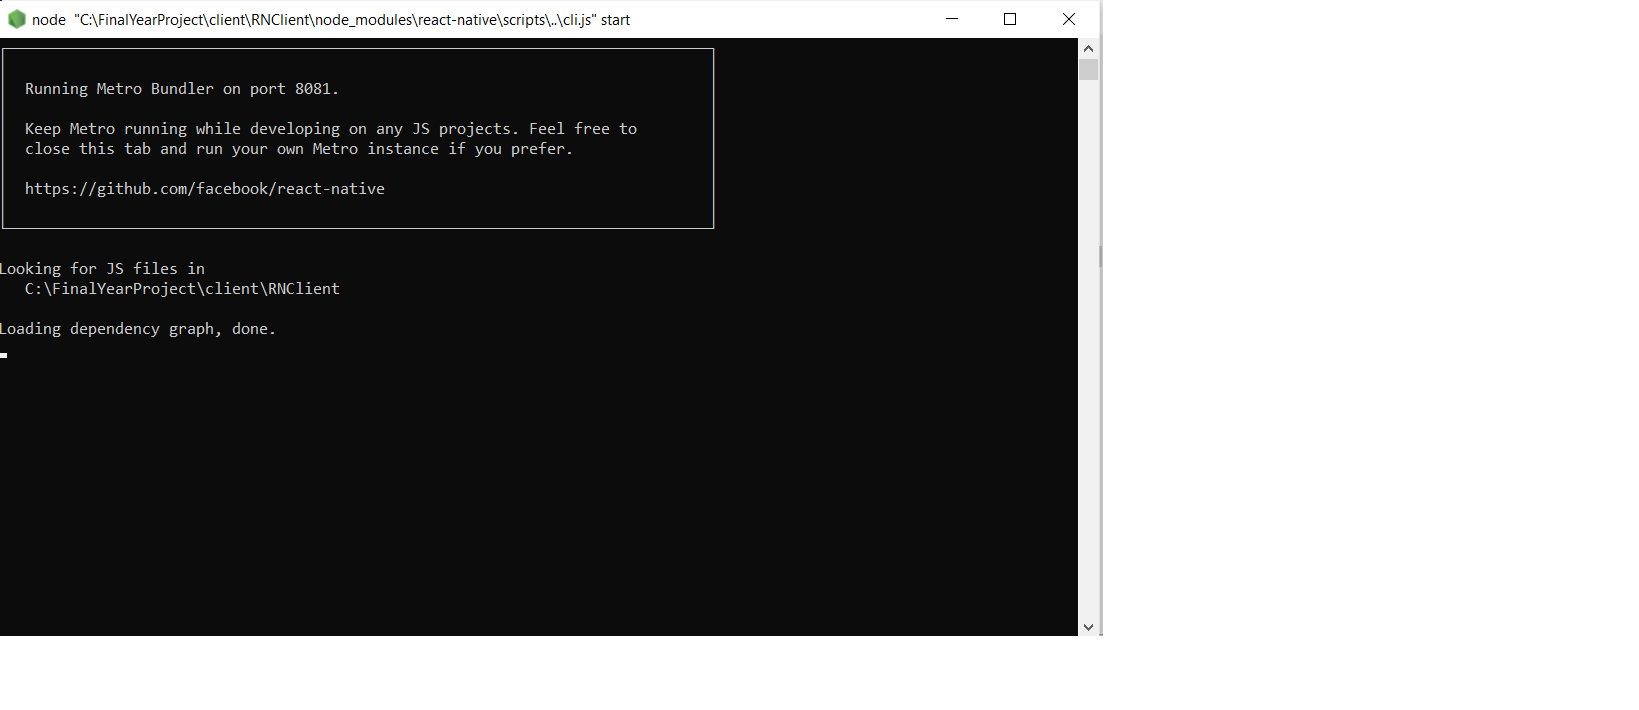
\includegraphics[width=1.9\textwidth]{img/metro.png}
     \caption{Metro Server}
    \label{fig:Metro}
\end{figure}

From time to time when a program doesn't compile and origin of the thrown errors cannot be identified the following command helps: 

\begin{lstlisting}
gradlew clean
\end{lstlisting}

